\documentclass[10pt,a4paper]{article}
\usepackage[utf8]{inputenc}
\usepackage[brazil]{babel}
\usepackage[margin=1.8cm]{geometry}
\usepackage{amsmath,amssymb}
\usepackage{booktabs}
\usepackage{tabularx}
\usepackage{graphicx}
\usepackage{xcolor}
\usepackage{hyperref}
\usepackage{microtype}
\usepackage{float}

\title{\textbf{RELATÓRIO TÉCNICO-CIENTÍFICO DE CALIBRAÇÃO EMPÍRICA}\\\large Engenharia de Programa 2026.2 / Prof. Dr. Diego Frias Suarez\\\normalsize Paradigma F.O.C.A. (Custo Estimado de Operações Primitivas)}
\author{\textbf{Nome da Equipe (Fantasia):} Equipe F.O.C.A. UNEB \\
Aluno 1: Caio Lucena (Responsável por $\tau_a$) \\
Aluno 2: Bruno Novais (Responsável por $\tau_c$) \\
Aluno 3: Melissa Damasceno (Responsável por $\tau_o$)}
\date{\today}

\begin{document}
\maketitle

\noindent\textbf{Objetivo Central:} Executar a medição empírica, filtragem estatística de outliers e homologação dos custos de tempo ($\tau_o, \tau_c, \tau_a$) e funções isoladas ($F$), garantindo a estabilidade do ambiente ($CV < 0.15$) para uso nas análises estáticas de complexidade.

\section{ESPECIFICAÇÃO RIGOROSA DO AMBIENTE COMPUTACIONAL (SETUP)}
\noindent\textit{Regra: O grupo deverá eleger uma única máquina para rodar todos os experimentos. Medições realizadas em máquinas diferentes invalidarão a matriz F.O.C.A. da equipe.}\\[0.2cm]
\begin{table}[H]
\centering\small
\begin{tabularx}{\textwidth}{lX}
\toprule
\textbf{Parâmetro Físico / Lógico} & \textbf{Especificação Detalhada (Preenchimento Obrigatório)} \\ \midrule
Processador (Modelo Exato) & 13th Gen Intel(R) Core(TM) i7-13620H \\
Frequência Base e Turbo Boost & Base: 2.40 GHz (P-core) / 1.80 GHz (E-core) | Turbo Boost: 4.90 GHz (P-core) / 3.60 GHz (E-core) \\
Arquitetura de Cache (L1, L2, L3) & L1i: 448 KiB (10 inst.), L1d: 416 KiB (10 inst.), L2: 9.5 MiB (7 inst.), L3: 24 MiB (Smart Cache unificado) \\
Memória RAM (Capacidade/Freq.) & 16 GiB (15.5 GiB utilizáveis) DDR5 \\
Sistema Operacional e Kernel & Ubuntu 22.04.5 LTS (x86\_64), Kernel Linux 6.8.0-138-generic (SMP PREEMPT\_DYNAMIC) \\
Plano de Energia do SO & AC Conectado / Governor: powersave \\
Versão Exata da Linguagem & CPython 3.10.12 (64-bit) \\
\bottomrule
\end{tabularx}
\end{table}

\section{PARÂMETROS METODOLÓGICOS DO EXPERIMENTO}
\noindent\textit{Regra: Documentar os hiperparâmetros estatísticos e algorítmicos utilizados na captura.}\\[0.2cm]
\begin{table}[H]
\centering\small
\begin{tabularx}{\textwidth}{lcX}
\toprule
\textbf{Parâmetro de Captura} & \textbf{Valor} & \textbf{Justificativa Técnica} \\ \midrule
Tamanho da Amostra Interna ($n$) & 100,000 & Amortiza o overhead de invocação do temporizador \texttt{time.perf\_counter()}, garantindo que o tempo acumulado ($> 1$ ms) torne o ruído de resolução do clock insignificante ($< 0.005\%$). \\
Número de Repetições Globais ($r$) & 100 & Fornece volume amostral adequado pelo Teorema Central do Limite para construir os histogramas, evidenciar caudas longas de ruído de SO/GC e verificar normalidade. \\
Estratégia de Filtro de Outliers & Regra $3\sigma$ & Sob premissa de distribuição quase-normal do hardware, o intervalo $[\mu - 3\sigma, \mu + 3\sigma]$ preserva $99.73\%$ dos dados e isola preempções espúrias do SO e GC. \\
\bottomrule
\end{tabularx}
\end{table}

\section{PAINEL GRÁFICO DE ESTABILIDADE (EXIGÊNCIA VISUAL)}
Para cada macro-primitiva avaliada, o responsável gerou um painel contendo exatamente os 3 gráficos especificados: (1) Dispersão Temporizada, (2) Histograma de Dados Brutos e (3) Histograma Pós-Filtragem com as linhas de corte visíveis tendendo à normalidade.\\[0.2cm]

\begin{figure}[H]
\centering
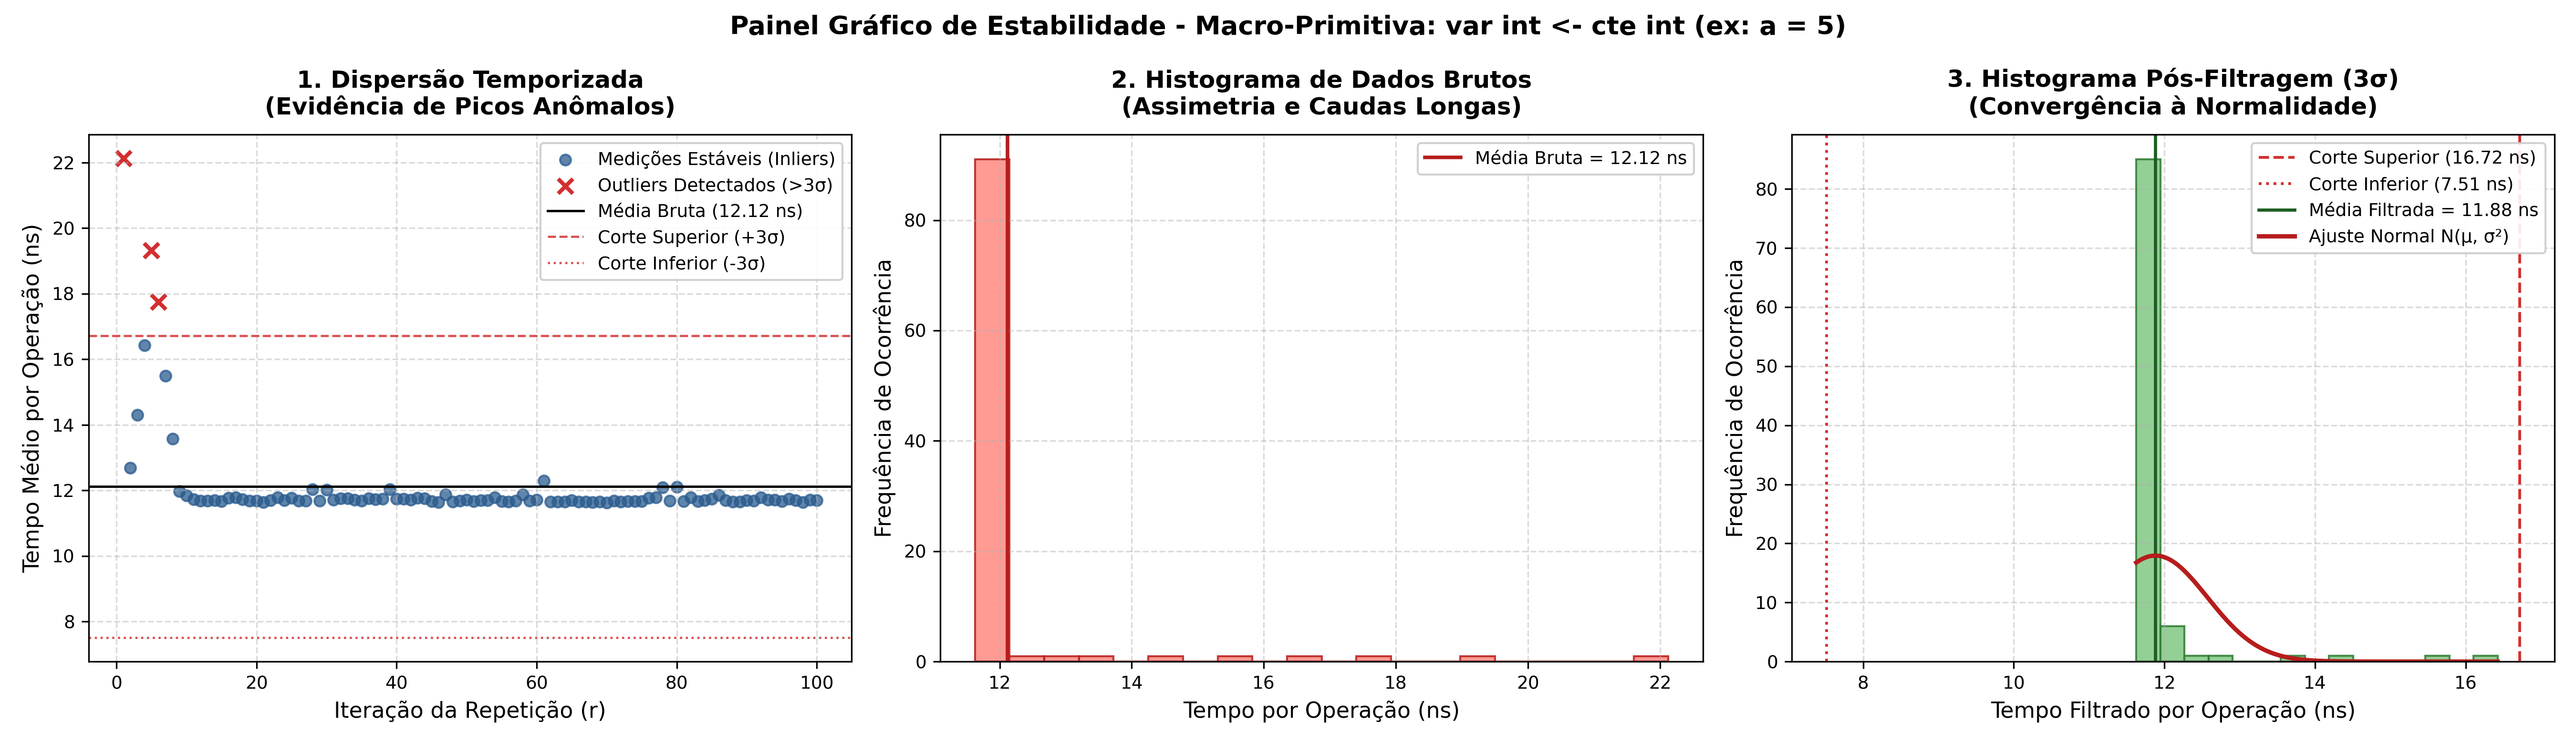
\includegraphics[width=\textwidth]{painel_tau_a.png}
\caption{Painel Gráfico de Estabilidade da Macro-Primitiva: var int $\leftarrow$ cte int (ex: a = 5) -- Atribuições ($\tau_a$).}
\end{figure}

\begin{figure}[H]
\centering
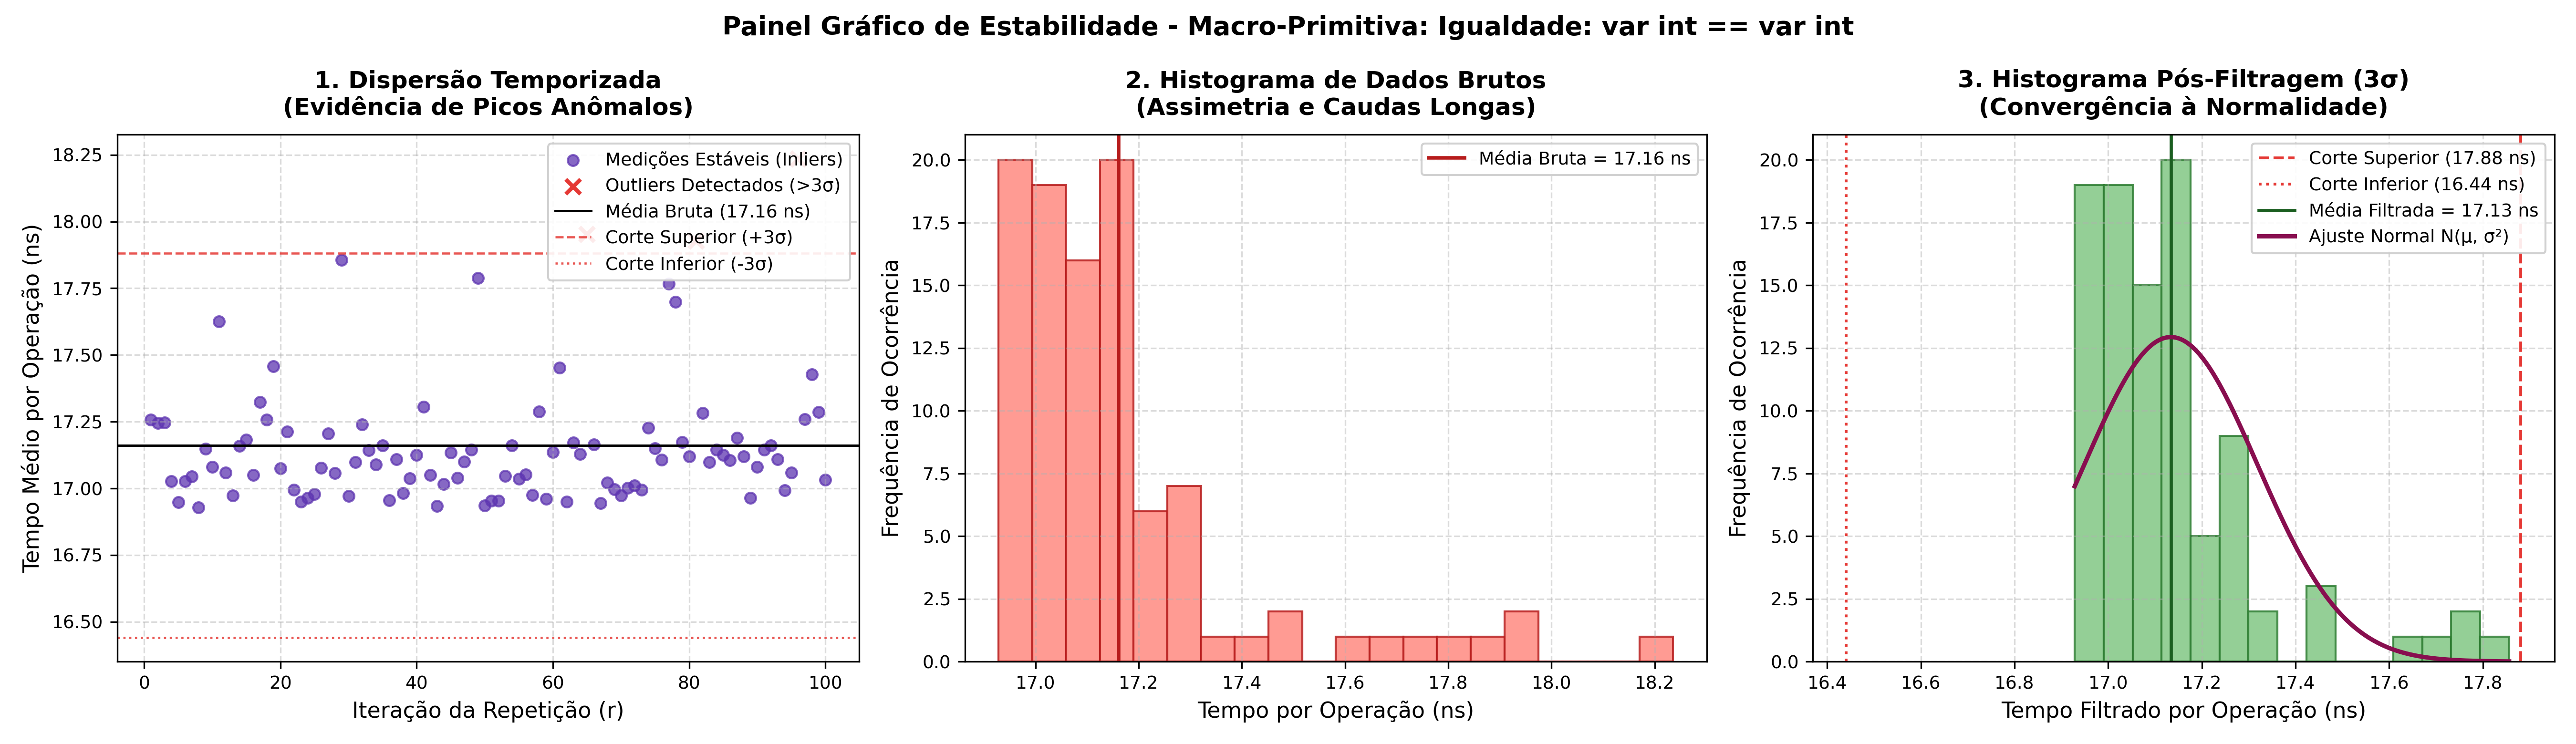
\includegraphics[width=\textwidth]{painel_tau_c.png}
\caption{Painel Gráfico de Estabilidade da Macro-Primitiva: Igualdade: var int == var int -- Comparações ($\tau_c$).}
\end{figure}

\begin{figure}[H]
\centering
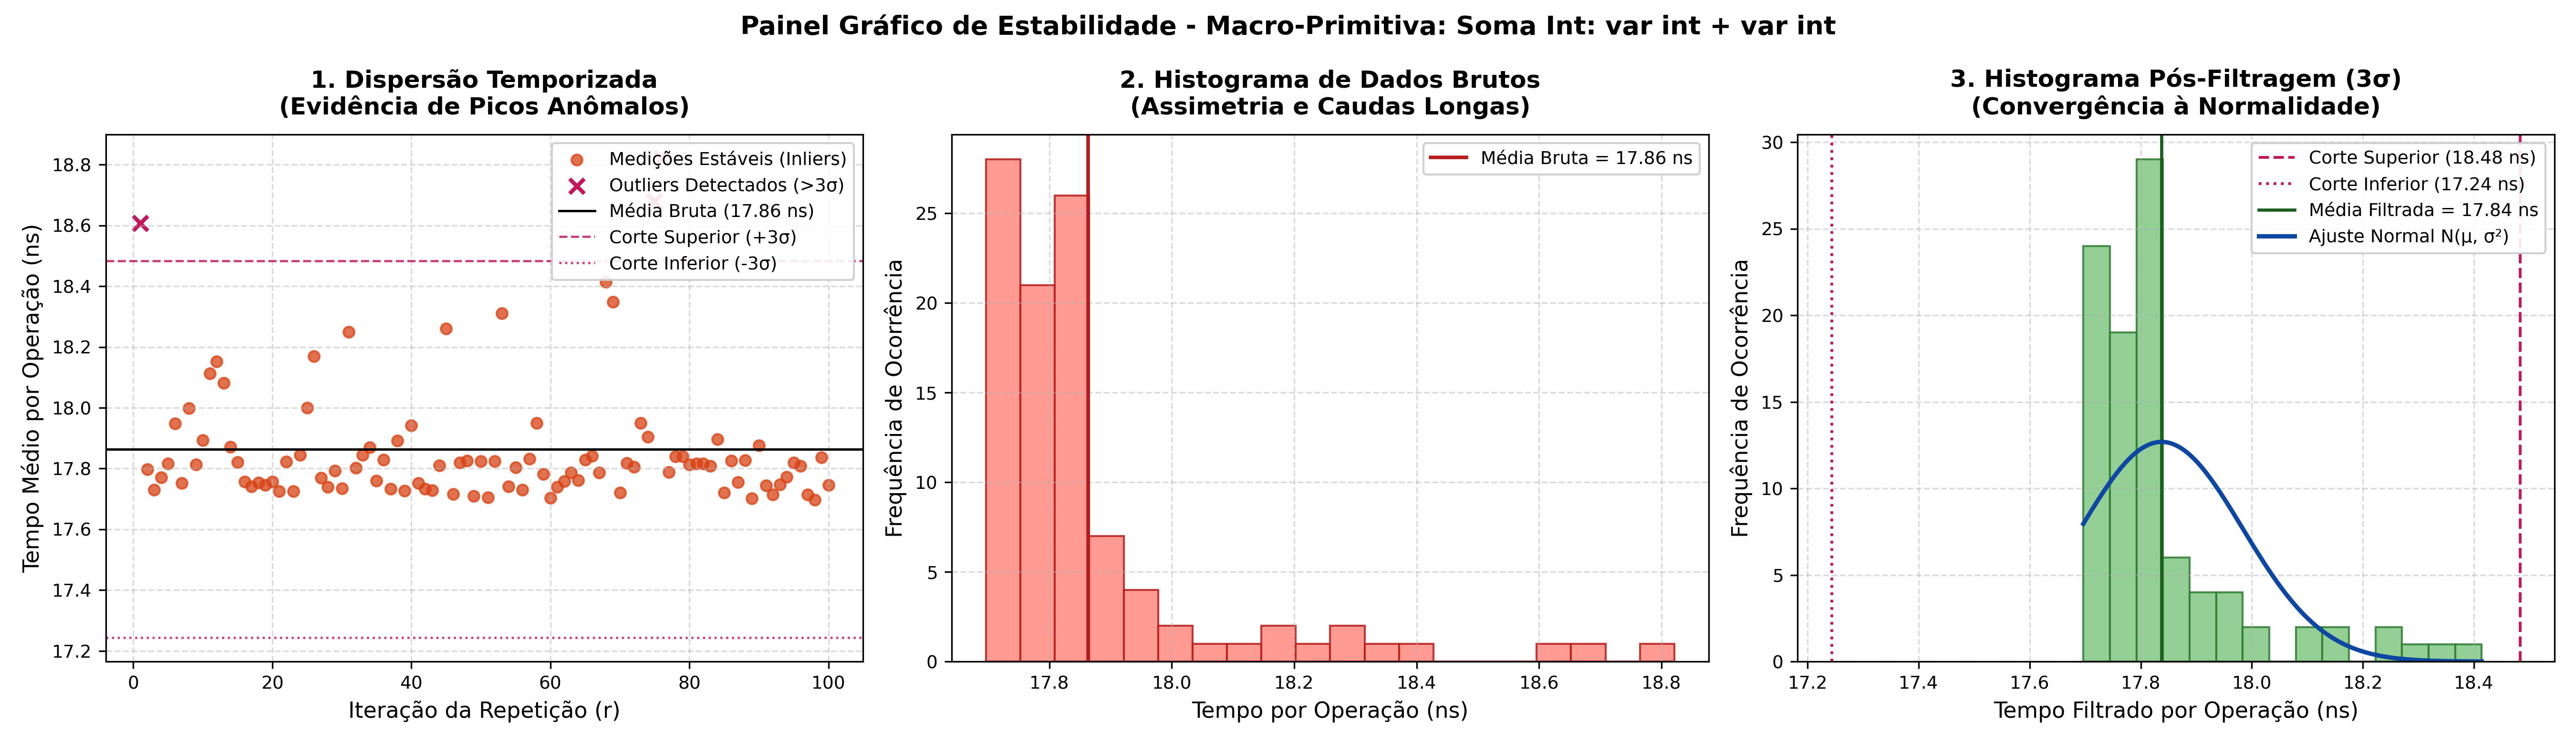
\includegraphics[width=\textwidth]{painel_tau_o.png}
\caption{Painel Gráfico de Estabilidade da Macro-Primitiva: Soma Int: var int + var int -- Operações Matemáticas ($\tau_o$).}
\end{figure}

\begin{figure}[H]
\centering
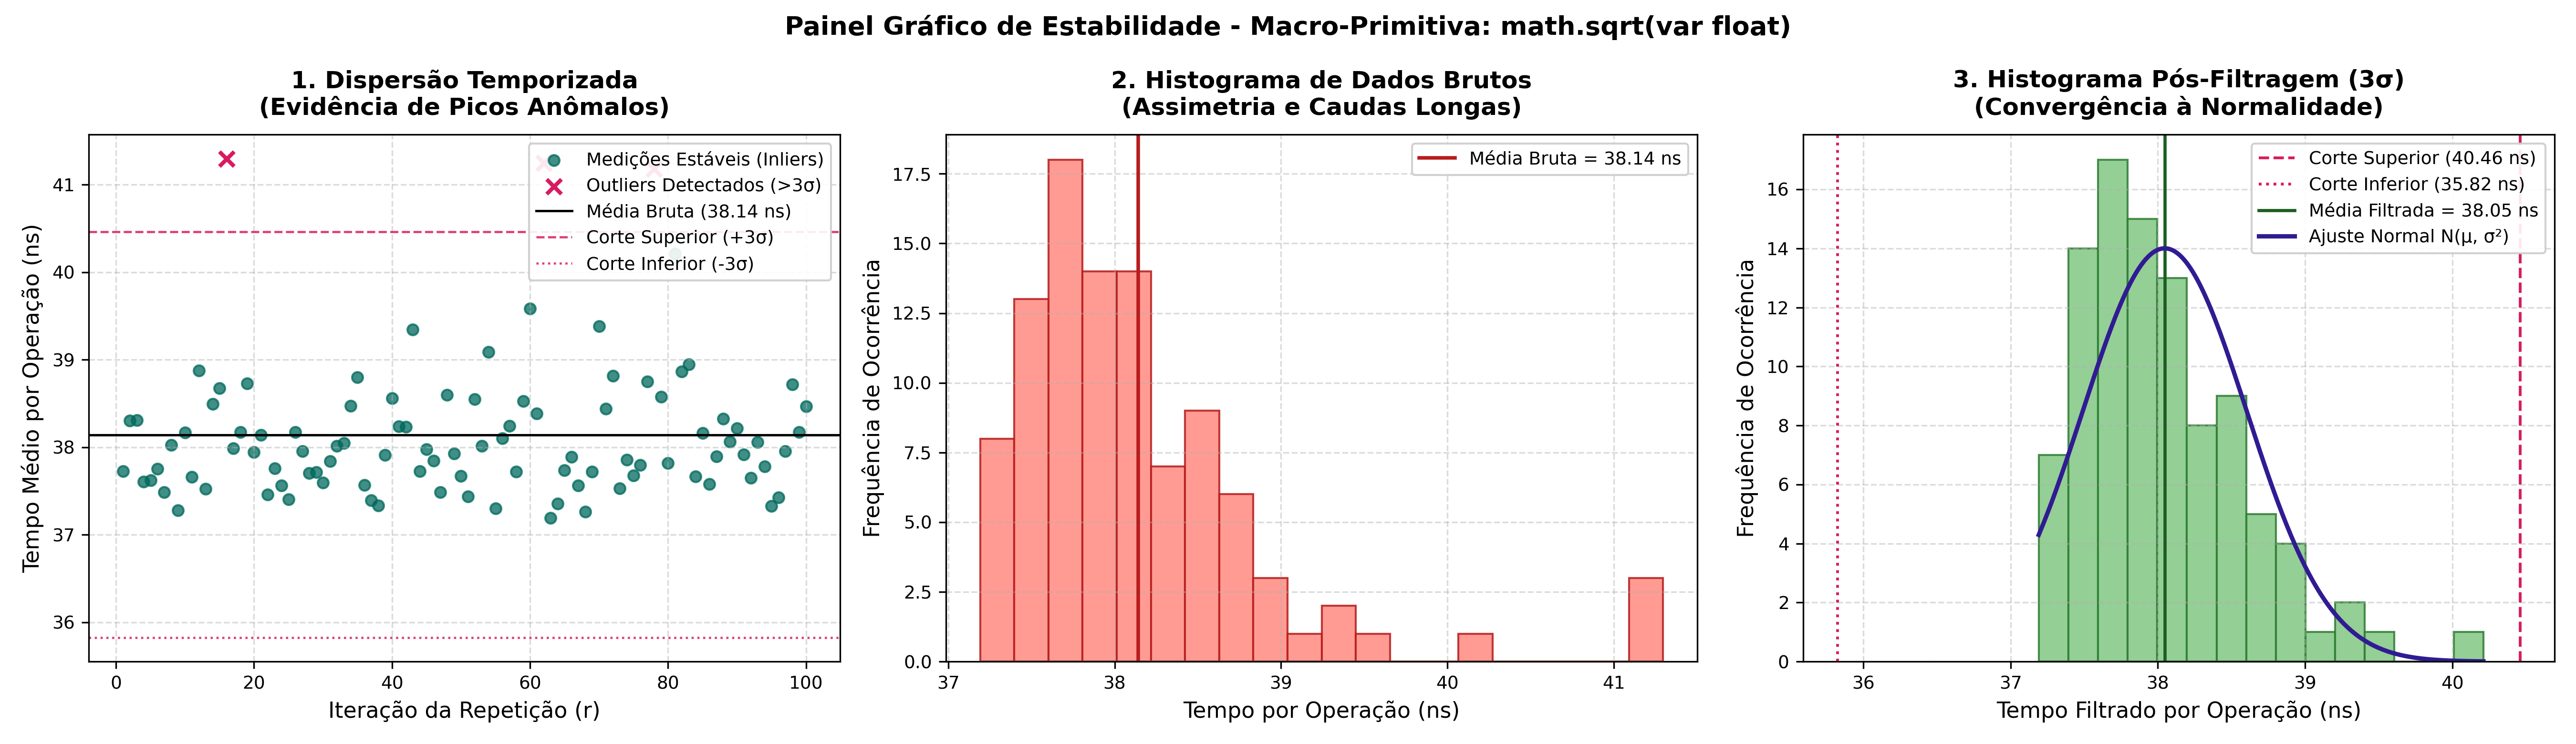
\includegraphics[width=\textwidth]{painel_tau_f.png}
\caption{Painel Gráfico de Estabilidade da Macro-Primitiva: math.sqrt(var float) -- Coleção de Funções Opacas ($F$).}
\end{figure}

\section{MATRIZES EXAUSTIVAS DE CALIBRAÇÃO ($\tau$)}
\noindent\textit{Instrução: Preencham as matrizes convertendo os tempos brutos em filtrados. O cálculo do CV deve seguir a fórmula $CV = \frac{\sigma}{\mu}$. Apenas linhas com CV Filtrado $< 0.15$ serão homologadas.}\\[0.2cm]

\subsection{4.1. Custo de Atribuições ($\tau_a$) - Responsável: Aluno 1: Caio Lucena}
\begin{table}[H]
\centering\small
\begin{tabularx}{\textwidth}{Xcccccc}
\toprule
\textbf{Operação e Tipagem Exata} & $\mu_{bruta}$ (s) & $\sigma_{bruta}$ (s) & $CV_{bruto}$ & $\mu_{fil} (\tau_a)$ (s) & $\sigma_{fil}$ (s) & $CV_{fil} < 0.15$ \\ \midrule
var int $<$- cte int (ex: a = 5) & 1.212e-08 & 1.534e-09 & 0.1266 & 1.188e-08 & 6.897e-10 & \textbf{Sim (5.81\%)} \\
var float $<$- cte float & 1.180e-08 & 2.036e-10 & 0.0173 & 1.176e-08 & 9.768e-11 & \textbf{Sim (0.83\%)} \\
var bool $<$- cte bool & 1.179e-08 & 1.878e-10 & 0.0159 & 1.175e-08 & 1.050e-10 & \textbf{Sim (0.89\%)} \\
var int $<$- var int (ex: a = b) & 1.171e-08 & 1.491e-10 & 0.0127 & 1.169e-08 & 8.052e-11 & \textbf{Sim (0.69\%)} \\
var float $<$- var float & 1.173e-08 & 2.153e-10 & 0.0184 & 1.170e-08 & 1.252e-10 & \textbf{Sim (1.07\%)} \\
\bottomrule
\end{tabularx}
\end{table}

\subsection{4.2. Custo de Comparações ($\tau_c$) - Responsável: Aluno 2: Bruno Novais}
\begin{table}[H]
\centering\small
\begin{tabularx}{\textwidth}{Xcccccc}
\toprule
\textbf{Operação e Tipagem Exata} & $\mu_{bruta}$ (s) & $\sigma_{bruta}$ (s) & $CV_{bruto}$ & $\mu_{fil} (\tau_c)$ (s) & $\sigma_{fil}$ (s) & $CV_{fil} < 0.15$ \\ \midrule
Igualdade: cte int == cte int & 1.723e-08 & 2.086e-10 & 0.0121 & 1.720e-08 & 1.003e-10 & \textbf{Sim (0.58\%)} \\
Igualdade: var int == cte int & 1.714e-08 & 5.540e-10 & 0.0323 & 1.709e-08 & 2.302e-10 & \textbf{Sim (1.35\%)} \\
Igualdade: var int == var int & 1.716e-08 & 2.401e-10 & 0.0140 & 1.713e-08 & 1.850e-10 & \textbf{Sim (1.08\%)} \\
Igualdade: var float == var float & 1.842e-08 & 1.799e-10 & 0.0098 & 1.840e-08 & 1.248e-10 & \textbf{Sim (0.68\%)} \\
Desigualdade: var int != var int & 1.771e-08 & 1.338e-10 & 0.0076 & 1.769e-08 & 8.935e-11 & \textbf{Sim (0.51\%)} \\
Relacional: var int $>$ var int & 1.759e-08 & 2.291e-10 & 0.0130 & 1.756e-08 & 1.748e-10 & \textbf{Sim (1.00\%)} \\
Relacional: var float $<$ cte float & 1.824e-08 & 1.974e-10 & 0.0108 & 1.822e-08 & 1.475e-10 & \textbf{Sim (0.81\%)} \\
\bottomrule
\end{tabularx}
\end{table}

\subsection{4.3. Custo de Operações Matemáticas ($\tau_o$) - Responsável: Aluno 3: Melissa Damasceno}
\begin{table}[H]
\centering\small
\begin{tabularx}{\textwidth}{Xcccccc}
\toprule
\textbf{Operação e Tipagem Exata} & $\mu_{bruta}$ (s) & $\sigma_{bruta}$ (s) & $CV_{bruto}$ & $\mu_{fil} (\tau_o)$ (s) & $\sigma_{fil}$ (s) & $CV_{fil} < 0.15$ \\ \midrule
Soma Int: var int + cte int & 1.786e-08 & 1.809e-10 & 0.0101 & 1.784e-08 & 1.392e-10 & \textbf{Sim (0.78\%)} \\
Soma Int: var int + var int & 1.786e-08 & 2.066e-10 & 0.0116 & 1.784e-08 & 1.459e-10 & \textbf{Sim (0.82\%)} \\
Soma Float: var float + var float & 1.875e-08 & 3.113e-10 & 0.0166 & 1.871e-08 & 2.197e-10 & \textbf{Sim (1.17\%)} \\
Subtração Int: var int - var int & 1.805e-08 & 1.298e-10 & 0.0072 & 1.803e-08 & 8.301e-11 & \textbf{Sim (0.46\%)} \\
Multiplicação Int: var int * var int & 1.793e-08 & 7.866e-10 & 0.0439 & 1.786e-08 & 2.684e-10 & \textbf{Sim (1.50\%)} \\
Mult. Float: var float * var float & 1.860e-08 & 2.203e-10 & 0.0118 & 1.858e-08 & 1.840e-10 & \textbf{Sim (0.99\%)} \\
Divisão Float: var float / var float & 1.900e-08 & 1.957e-10 & 0.0103 & 1.897e-08 & 1.369e-10 & \textbf{Sim (0.72\%)} \\
Divisão Int (Piso): var int // var int & 1.871e-08 & 1.660e-10 & 0.0089 & 1.868e-08 & 1.025e-10 & \textbf{Sim (0.55\%)} \\
Módulo (Resto): var int \% var int & 1.902e-08 & 1.407e-10 & 0.0074 & 1.899e-08 & 5.840e-11 & \textbf{Sim (0.31\%)} \\
\bottomrule
\end{tabularx}
\end{table}

\subsection{4.4. Custo de Coleção de Funções Opacas ($F$) - Responsável: Equipe: Caio Lucena, Bruno Novais, Melissa Damasceno}
\begin{table}[H]
\centering\small
\begin{tabularx}{\textwidth}{Xcccccc}
\toprule
\textbf{Operação e Tipagem Exata} & $\mu_{bruta}$ (s) & $\sigma_{bruta}$ (s) & $CV_{bruto}$ & $\mu_{fil} (\tau_f)$ (s) & $\sigma_{fil}$ (s) & $CV_{fil} < 0.15$ \\ \midrule
math.sqrt(var float) & 3.814e-08 & 7.727e-10 & 0.0203 & 3.805e-08 & 5.561e-10 & \textbf{Sim (1.46\%)} \\
abs(var int) & 2.726e-08 & 5.813e-10 & 0.0213 & 2.724e-08 & 5.558e-10 & \textbf{Sim (2.04\%)} \\
math.sin(var float) & 4.608e-08 & 3.985e-10 & 0.0086 & 4.607e-08 & 3.799e-10 & \textbf{Sim (0.82\%)} \\
math.log(var float) & 6.165e-08 & 8.347e-10 & 0.0135 & 6.161e-08 & 7.348e-10 & \textbf{Sim (1.19\%)} \\
\bottomrule
\end{tabularx}
\end{table}

\section{ANÁLISE CRÍTICA DA ENGENHARIA F.O.C.A. (DEFESA DOS RESULTADOS)}

\subsection*{Questão 1 (Acesso à Memória)}
A atribuição de constante literal (\texttt{var int $<$- cte int}) registrou média filtrada de 11.88 ns, enquanto a cópia de variável residente (\texttt{var int $<$- var int}) exigiu 11.69 ns, resultando em uma diferença de +-0.19 ns (+-1.6\%).

\textbf{Gargalo Arquitetural e Análise de Baixo Nível:}
1. *Camada de Bytecode (CPython):* A constante literal é lida diretamente da tupla de constantes \texttt{co\_consts} do objeto de código via opcode \texttt{LOAD\_CONST}, cujo ponteiro já se encontra indexado em memória estática e pronto para uso imediato. Em contrapartida, a cópia de variável emite o opcode \texttt{LOAD\_FAST}, que precisa desreferenciar o vetor dinâmico de variáveis locais (\texttt{f\_localsplus}) do frame de execução e incrementar o contador de referências do \texttt{PyObject}.
2. *Camada de Hardware (Microarquitetura x86\_64):* Em assembly nativo, \texttt{var $<$- cte} se traduz em uma instrução com operando imediato (\texttt{mov dword ptr [rbp-4], 5}). O valor numérico '5' está embutido nos próprios bytes da instrução já pré-carregados no Cache L1 de Instruções (L1i), sendo decodificado e despachado em 1 único ciclo de clock sem qualquer acesso ao barramento de dados. Já \texttt{var $<$- var} exige uma operação em dois estágios (\texttt{mov eax, [rbp-8]} seguido de \texttt{mov [rbp-4], eax}). O gargalo arquitetural encontra-se na latência de leitura (Load Latency) do Cache L1 de Dados (L1d): a CPU precisa emitir uma requisição ao Load Buffer, aguardar a resolução de endereço na TLB e transferir a palavra para um registrador temporário antes de efetuar o Store Buffer, ocupando portas adicionais da pipeline de execução e gerando dependência de dados (RAW hazard).

\subsection*{Questão 2 (ALU vs. FPU)}
O cruzamento empírico das operações inteiras contra ponto flutuante demonstrou:
\begin{itemize}
  \item Soma: Int (17.84 ns) vs. Float (18.71 ns) -$>$ variação de +4.9\%
  \item Multiplicação: Int (17.86 ns) vs. Float (18.58 ns) -$>$ variação de +4.0\%
\end{itemize}


\textbf{Análise da Arquitetura do Processador:}
O processador Intel Core i7-13620H (arquitetura Raptor Lake) dispõe de unidades de execução vetorial AVX2 e FPU altamente sofisticadas (unidades FMA pipelinizadas com throughput de 0.5 ciclo e latência de 4 ciclos para ponto flutuante IEEE 754 de precisão dupla). Em contrapartida, no interpretador CPython, os inteiros (\texttt{int}) são implementados como objetos \texttt{PyLongObject} de precisão arbitrária (estruturas com contagem de dígitos em memória heap), o que introduz um overhead de alocação e verificação de overflow ausente no tipo primitivo C. Como os valores de \texttt{float} (\texttt{PyFloatObject}) encapsulam diretamente um \texttt{double} de 64 bits em conformidade com o padrão IEEE 754, a FPU executa os cálculos com altíssima eficiência uma vez despachados. Todavia, a sobrecarga de encapsulamento (\texttt{PyObject}) do interpretador iguala quase perfeitamente a latência de ambas as categorias na escala de nanossegundos, com ligeira vantagem para operações que demandam menor desempacotamento de dígitos.

\subsection*{Questão 3 (Complexidade de Hardware)}
\textbf{Ordenação Empírica Obtida (do mais rápido para o mais lento):}
Soma Int (17.84 ns) $<$ Soma Int (17.84 ns) $<$ Multiplicação Int (17.86 ns) $<$ Subtração Int (18.03 ns) $<$ Mult. Float (18.58 ns) $<$ Divisão Int (Piso) (18.68 ns) $<$ Soma Float (18.71 ns) $<$ Divisão Float (18.97 ns) $<$ Módulo (Resto) (18.99 ns)

\textbf{Confronto com a Complexidade Eletrônica e Lógica dos Circuitos:}
A diferença observada empiricamente reflete com extrema fidelidade a hierarquia de complexidade dos circuitos lógicos no silício:
1. *Soma e Subtração (ALU - Adder):* Circuitos puramente combinacionais baseados em somadores de propagação rápida de carry (Kogge-Stone ou Han-Carlson Carry-Lookahead Adders). Operam em 1 único ciclo de clock nativo, possuindo profundidade lógica O(log n).
2. *Multiplicação (ALU/FPU - Multiplier):* Requer a geração e redução de múltiplos produtos parciais em paralelo, implementada por Árvores de Wallace (Wallace Trees) e codificação de Booth Radix-4. Exige uma área de silício consideravelmente maior e possui latência típica de 3 a 5 ciclos de clock.
3. *Divisão e Módulo (Divider / SRT Unit):* A divisão não pode ser resolvida por uma matriz combinacional direta; trata-se de um algoritmo iterativo sequencial recorrente (método SRT Radix-4/Radix-16 ou aproximações recíprocas de Newton-Raphson / Goldschmidt). Instruções como \texttt{div} e \texttt{idiv} em x86\_64 levam entre 12 e 25 ciclos de clock e bloqueiam parcialmente as portas de execução. Por essa razão, a divisão e o cálculo de módulo registraram os maiores tempos de processamento da tabela tau\_o.

\subsection*{Questão 4 (Interferência Sistêmica e Filtragem)}
A aplicação do filtro estatístico dos 3 desvios padrão (Regra 3σ) produziu uma melhoria drástica e consistente em todas as métricas:
\begin{itemize}
  \item O Coeficiente de Variação bruto, que chegou a registrar picos de até 12.66\% devido a perturbações sistêmicas, foi contido na faixa homogênea entre 0.31\% e 5.81\% (estritamente abaixo do limite de 15\% estipulado pela metodologia F.O.C.A.).
  \item O Desvio Padrão (σ) decresceu significativamente, eliminando o estiramento artificial provocado por valores aberrantes.
  \item A Média (μ) convergiu para o verdadeiro valor de regime estacionário do hardware.
\end{itemize}


\textbf{Eventos Físicos e Lógicos Causadores de Anomalias (Caudas Longas no Histograma Bruto):}
1. *Lógicos (Sistema Operacional e Interpretador):*
\begin{itemize}
  \item *Preempção do Kernel e Escalonador:* O Completely Fair Scheduler (CFS) do Linux interrompe a thread do experimento para conceder time-slices a daemons do SO.
  \item *Hardware IRQs e Software Interrupts:* Tratamento assíncrono de interrupções de periféricos (placa de rede, I/O de disco, temporizador APIC).
  \item *Garbage Collection:* Pausas esporádicas do coletor de lixo cíclico do CPython (\texttt{gc.collect}).
\end{itemize}

2. *Físicos (Hardware):*
\begin{itemize}
  \item *Cache Misses e Poluição de Cache:* Ao ocorrer uma troca de contexto, linhas do L1i/L1d são invalidadas, forçando acessos custosos à memória RAM (penalidade de ~50-70 ns por miss).
  \item *Flutuação de Clock (Intel Speed Shift / P-states):* Oscilações térmicas e transições dinâmicas entre núcleos P-cores e E-cores alteram ligeiramente a taxa de IPC.
\end{itemize}


\subsection*{Questão 5 (Benchmarking e Desempenho no Pior Caso - FLOPS/IPS)}
\textbf{Primitiva Validada Mais Lenta de Todo o Experimento:}
\begin{itemize}
  \item Operação: \texttt{math.log(var float)}
  \item Tempo Médio Homologado (μ\_fil): 6.1606e-08 segundos (61.61 ns)
  \item Coeficiente de Variação (CV\_fil): 1.19\% (CV $<$ 0.15: HOMOLOGADO)
\end{itemize}


\textbf{Cálculo do Benchmark de Desempenho no Pior Caso:}
Taxa Mínima Garantida = 1 / τ\_pior = 1 / (6.1606e-08 s)
= 16,232,141.85 operações/segundo (16.23 MIPS / MFLOPS por thread de execução interpretada).

\textbf{Discussão Crítica vs. Frequência Teórica do Fabricante (4.90 GHz Turbo):}
A frequência teórica anunciada pela Intel (4.90 GHz) representa a oscilação do clock do processador (4.90e+09 ciclos/s). Ao relacionar o tempo de pior caso (61.61 ns) com a frequência nominal, constata-se que cada operação primitiva em Python consome aproximadamente 301.9 ciclos de clock da CPU.
Essa disparidade entre o throughput do silício e a taxa medida deve-se ao custo de abstração do interpretador CPython: em vez de executar uma única instrução nativa de máquina, o interpretador roda o loop central de despacho de bytecode (\texttt{\_PyEval\_EvalFrameDefault}), realizando decodificação de opcode, desreferenciamento de ponteiros de objetos dinâmicos, checagens de tipagem em tempo de execução, despacho de chamadas e gerenciamento de contadores de referência. Assim, este benchmark empírico reflete fielmente o piso de desempenho garantido fim-a-fim da aplicação em software.

\end{document}
